\section{Simulation d'un système de freinage sans ABS}
Durant la pratique des travaux sur VHDL-AMS il est demandé aux étudiants de réaliser et d'instancier étapes par étapes les différentes partie d'un système de freinage d'une voiture. Pour la réalisation du travail nous avons travailler avec le logiciel ModelSim et un éditeur de texte pour venir rédiger, en VHDL, les différentes instances du véhicule jusqu'à l'intégration de l'ABS.

\begin{figure}[h]
    \centering
    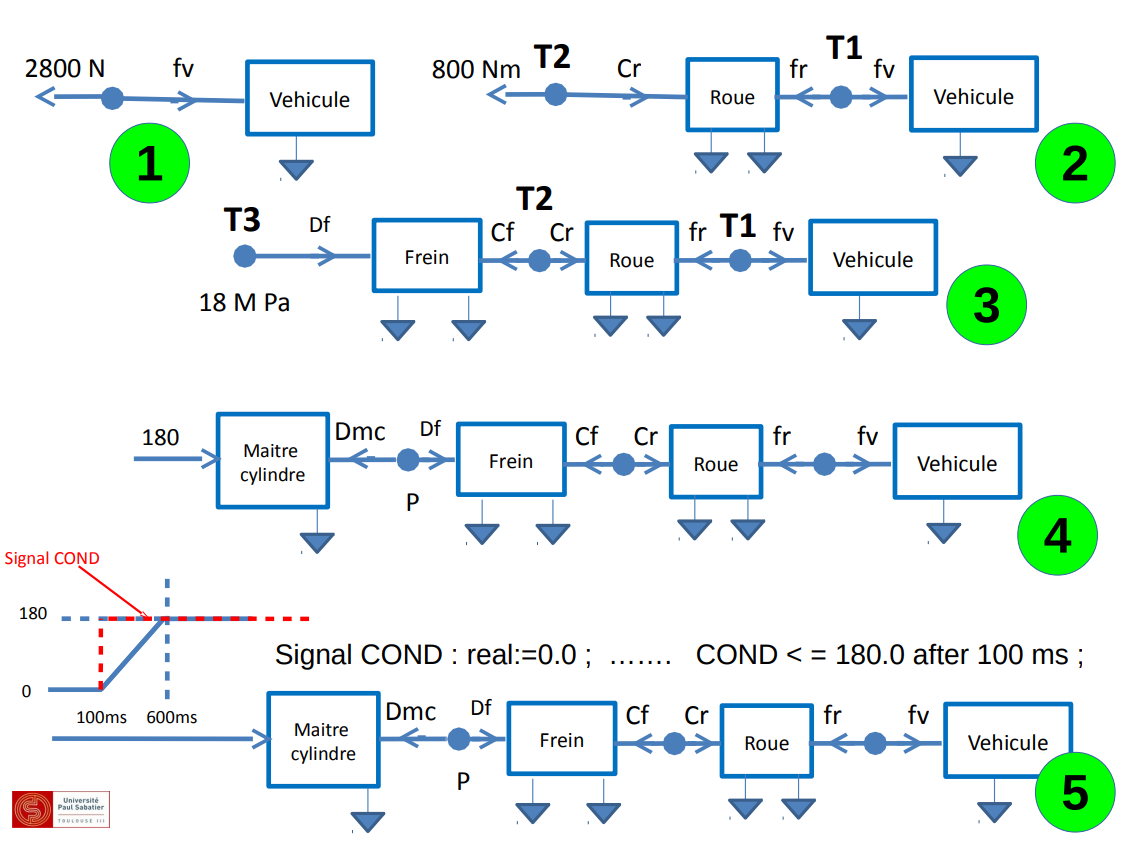
\includegraphics[width=\textwidth]{images/etapes.png}
    \caption{Implémentation des différentes parties du système de freinage d'une voiture}
\end{figure}

Il est demandé d'instancier étapes par étapes différents blocs avec leurs terminaux coresspondants, comme indiqué dans le powerpoint de présentation du TP.

\newpage

\subsection{Analyse instanciation véhicule }
Dans cette première partie nous devons instancier le véhicule fournit dans les fichiers du projet. Sur la Figure 2 on peut voir le schéma bloc qu'il faut instancier et décrire par la suite son entitée en VHDL-AMS.

\begin{figure}[h]
    \centering
    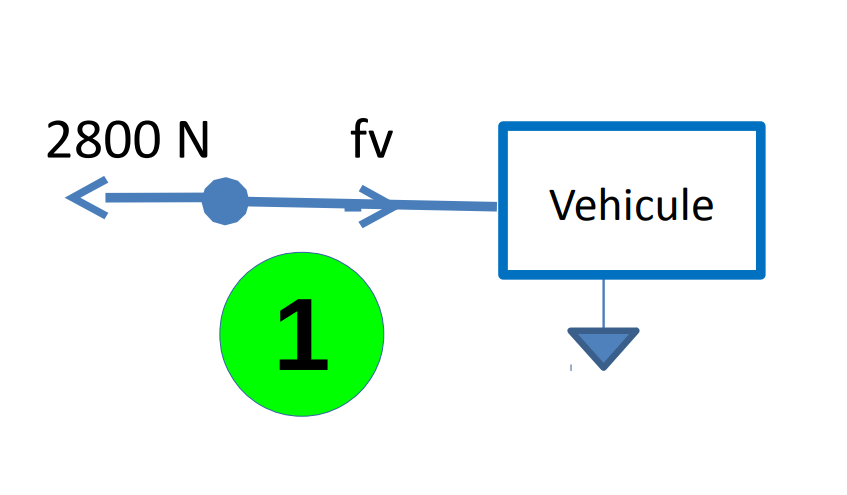
\includegraphics[width=0.5\textwidth]{images/un.png}
    \caption{Instanciation du véhicule avec son terminal}
\end{figure}

Dans l'entitée du véhicule nous avons donc à définir certaines quantités qui va nous permettra de résoudre certaines équations :\\

\begin{itemize}
        \item $m        \rightarrow$ Masse véhicule.
        \item $Cx       \rightarrow$ Coefficient aérodynamique.
        \item $S        \rightarrow$ Surface Frontale.
        \item $V\_init  \rightarrow$ Vitesse initiale du vehicule.
\end{itemize}

\begin{figure}[h]
    \centering
    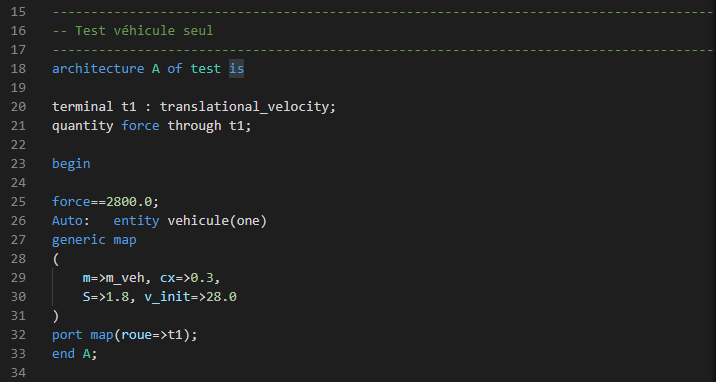
\includegraphics[width=\textwidth]{images/vehicule.png}
    \caption{Code VHDL Architecture A - Véhicule}
\end{figure}

Pour la première partie, véhicule il faudra mettre en place un terminal T1 ayant pour type "Translational\_velocity". Celui-ci sera plus tard rélié au Terminal "Roue", du même type, pour nous permettre la visualisation de la vitesse du véhicule.
\newpage
Avec l'aide du logiciel ModelSim nous pouvons simuler le temps de freinage nécessaire à l'arrêt du véhicule lorsqu'on lui applique une force de 2800 N au terminal T1.

\begin{figure}[h]
    \centering
    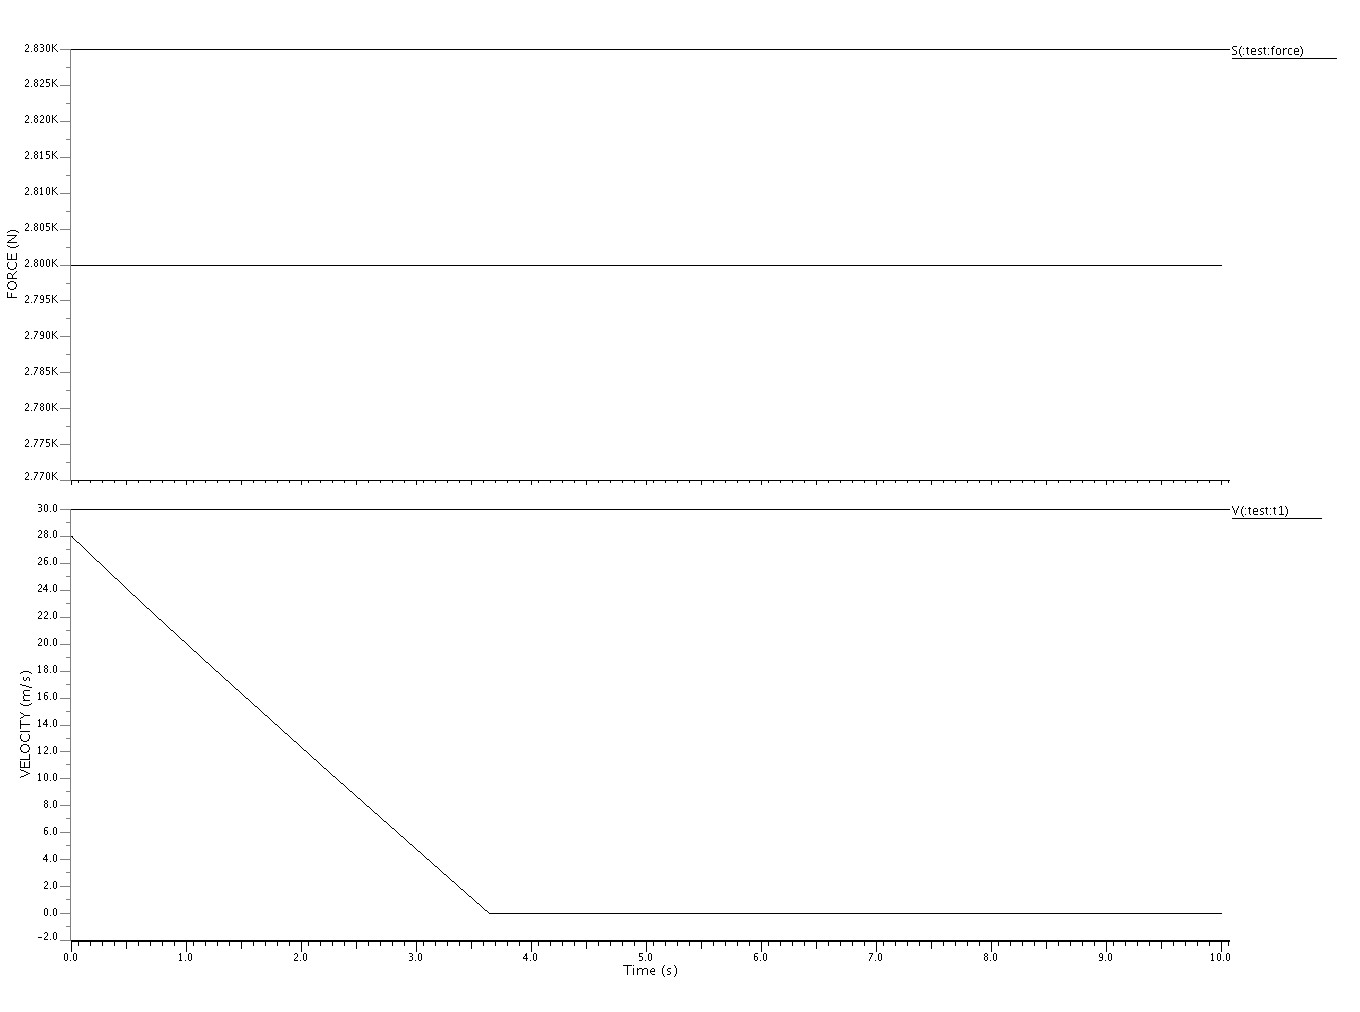
\includegraphics[width=\textwidth]{images/Instanciation_vehicule.jpg}
    \caption{Simulation Terminal T1 Force et Temps pour le freinage}
\end{figure}

\subsection{Analyse instanciation roue}
Une fois le véhicule instancié on nous demande d'ajouter le système "Roue". Dans cette partie on déclare en code la partie générique suivante :\\
\begin{itemize}
    \item $route       \rightarrow$ Etat de la route (mouillée, seche).
    \item $m       \rightarrow$ Masse vehicule.
    \item $rR        \rightarrow$ Rayon de la roue.
    \item $IR  \rightarrow$ Inertie de la roue.
    \item $mu0_D \rightarrow$ Coéfficient adhérence sans glissement sur sol sec.
    \item $As \rightarrow$ Facteur de decroissance de l'adherence.
    \item $mu0_W \rightarrow$ Coéfficient adhérence sans glissement sur sol mouillé.
    \item $Vc \rightarrow$ Caracteristique de la surface.
\end{itemize}
\newpage

Dans cette partie du code il y aura deux terminaux à instancier au niveau de la roue :\\

\begin{itemize}
    \item $veh  \rightarrow $ De type "translational\_velocity".
    \item $frein    \rightarrow $ De type "rotational\_velocity".
\end{itemize}

\begin{figure}[h]
    \centering
    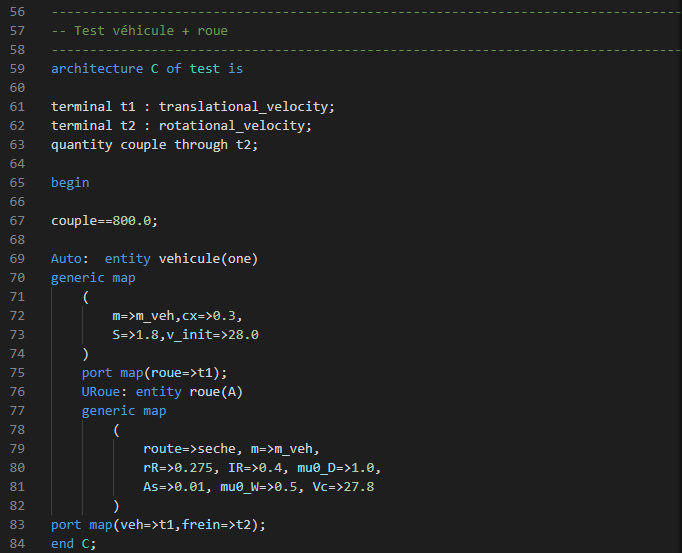
\includegraphics[width=\textwidth]{images/Roue.png}
    \caption{Code VHDL Architecture C - Roue}
\end{figure}

\newpage

Une fois la "Roue" implémentée on se retrouve sur ModelSim avec deux Terminaux, T2 étant le dernier terminal instancié qui représente le terminal d'entrée de "Roue" et T1 son Terminal de sortie. On observe grâce à ModelSim la vitesse rotationnelle de "Roue" ainsi que la vitesse du véhicule. On observe que la vitesse de "Roue" chute brusquement avant de réduire linéairement comme la vitesse du véhicule.

\begin{figure}[h]
    \centering
    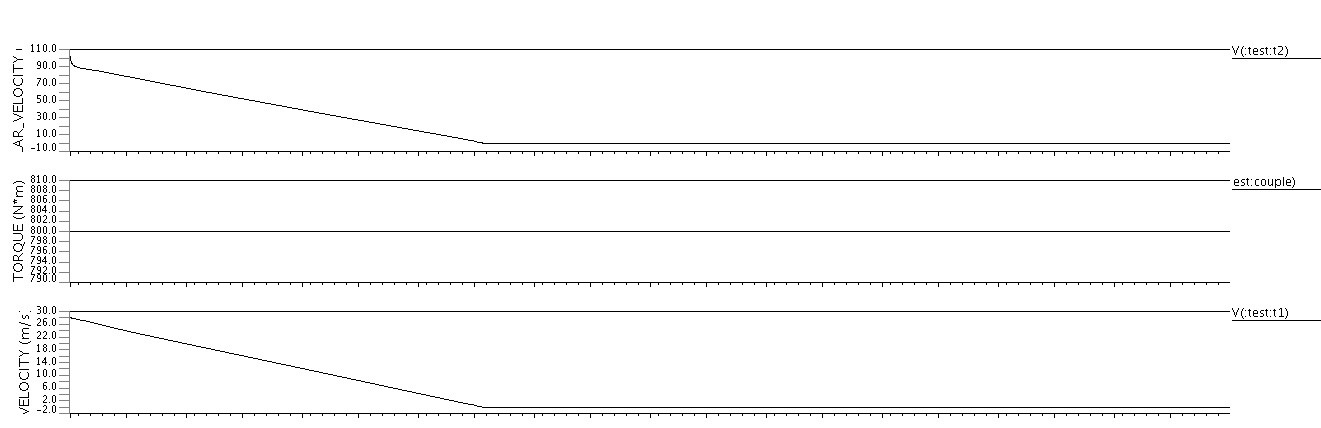
\includegraphics[width=1.1\textwidth]{images/Instanciation_roue.jpg}
    \caption{Simulation Terminal T2 et T1}
\end{figure}

\subsection{Analyse instanciation frein}
Une fois le véhicule et la Roue instanciés on nous demande d'ajouter le système "Frein". Dans cette partie on déclare en code la partie générique suivante :\\
\begin{itemize}
    \item $coef_fric    \rightarrow$ Coéfficient de friction des plaquettes.
    \item $S    \rightarrow$ Surface piston = 10 cm2.
    \item $R   \rightarrow$ Rayon moyen du disque.
\end{itemize}

Dans cette partie du code il y aura deux terminaux à instancier au niveau de la du Frein :

\begin{itemize}
    \item $Roue    \rightarrow$ Type "rotational\_velocity".
    \item $MC    \rightarrow$ Type "fluidic" à l'entrée du Frein.
\end{itemize}

Dans cette nouvelle instance nous venons d'implémenter le "Frein" permettant l'obtention de la vitesse de rotation du disque dans le terminal 2 en fonction de la pression appliquée à son entrée. On définit une quatité de Pression (across) et débit (Through) pour le nouvel Terminal. On vient ensuite fixer la valeur de pression à 18 MPa pour pouvoir résoudre l'équation.

\newpage

\begin{figure}[h]
    \centering
    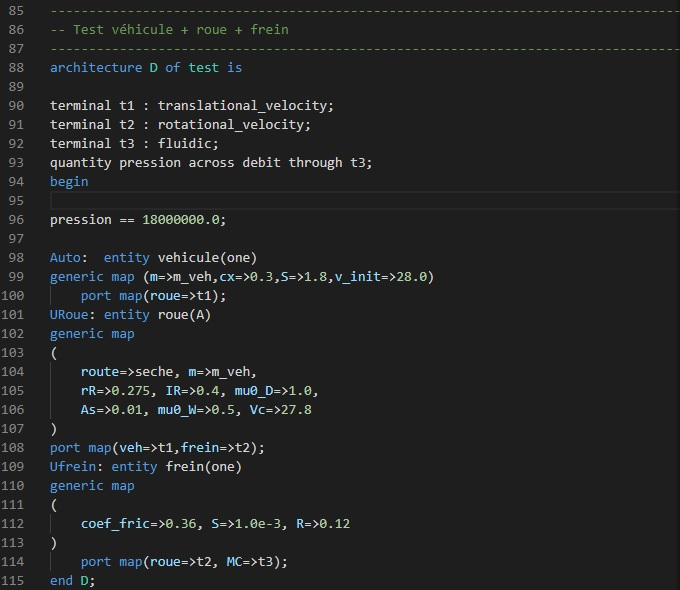
\includegraphics[width=0.85\textwidth]{images/Instanciation_frein.jpg}
    \caption{Code VHDL Architecture D - Roue}
\end{figure}


\newpage

\subsection{Analyse instanciation maître cylindre}
a
\subsection{Modélisation du régulateur de pression}
a
\newpage